\documentclass[parskip=half]{scrartcl}
\usepackage{hyperref}
\usepackage{graphicx}
\usepackage{subfig}
\usepackage{amsmath, amssymb}

\graphicspath{{./images/}}

\title{Explainable SVM}
\subtitle{Online Visualizations for Teaching}

\author{
  Hendrik Pfaff, Luca Jordan, Lukas Atkinson, Yasemin Er
  \\
  {\normalsize\ttfamily \{hendrik.pfaff,gian.jordan,atkinson,yasemin-\}@stud.fra-uas.de}
}

\date{Summer Term 2020}

\publishers{Frankfurt University of Applied Sciences}

\subject{Project Documentation}

\begin{document}
\maketitle

\section{Introduction}
As part of the digitalization project “Webtools for teaching” at Frankfurt University of Applied Sciences (FRA UAS), students of the general computer science Masters’ program created a website about one of the most common techniques used for regression- and classification problems, the Support Vector Machine (SVM). 
The SVM is very common these days and is used as a standard tool for text categorization, image recognition, hand-written digit recognition and bioinformatics.

In order to teach algorithms, interactive visualizations can be a powerful tool.
We therefore developed an interactive, web-based tool
to explain how Support Vector Machines (SVM) work.

\section{Support Vector Machines}
The SVM is a supervised learning model. In this approach, we are given a set of input vectors ($x_n$) paired with corresponding target values ($t_n$). 
The goal is to “learn” a model made out of these training set to make correct predictions of a target value $t$ for newly presented input data $x$. 
To “learn” a model means finding a hyperplane,
which is the set of points satisfying the hyperplane equation: $w*x+b = 0$,
where w is the weight vector, $x$ is the input vector and $b$ is the bias.

The hyperplane separates our training data into two classes which means that data points from one class are above the hyperplane and data points from the other class are below the hyperplane. 
There are several possible hyperplanes. The question, therefore, is which hyperplane best separates our data? The best hyperplane is the one that maximizes the margin. The margin is the shortest distance from the hyperplane to their closest points. 
So for describing the hyperplane mathematically it is not important to consider all training vectors but only those that are closest to the hyperplane. These vectors are called support vectors. 

The goal is to determine the parameters $w$ and $b$ of the optimal hyperplane, the hyperplane with the largest margin. In other words, we need to maximize the margin and maximizing the margin is an optimization problem that is equivalent to minimizing the norm of the weight vector $||w||$. 

In general, the norm of a vector $x = (x_1,...,x_N)$ is computed by using the euclidean norm formula: 

\[||w||=\sqrt{x_{1}^{2}+...+x_{N}^{2}}\]

Expressed mathematically, we have to solve the following optimization problem by adjusting the parameters $\mathbb w$, $b$: 
\begin{equation}
  \min \frac{1}{2}||w||^{2}
  \quad \text{subject to } y_i(w \cdot x_i) + b \ge 1 \forall i
  \label{eq:opt}
\end{equation}

This is a constrained optimization problem and such problems were solved by
efficient methods, such as the Lagrangian multiplier method.

\begin{align*}
  \mathcal L(\mathbf w, b, \alpha)
  &= f(\mathbf w) - \sum_{i=1}^m \alpha_i g_i(\mathbf w, b) \mathcal L(\mathbf w, b, \alpha)
  \\
  &= \frac 1 s ||\mathbf w||^2 - \sum_{i=1}^m \alpha_i \left(
      y_i(\mathbf w \cdot \mathbf x_i + b) - 1
    ) \right)
\end{align*}
\[
  \min_{\mathbf w, b} \max_\alpha \mathcal L(\mathbf w,b,\alpha)
  \quad \text{subject to } \alpha_i \ge 0 \forall i
\]

Vapnik and Cortes modified the original SVM to the Soft Margin SVM which means, in the classification case, outliers are allowed. The original optimization problem from \eqref{eq:opt} has been changed to \eqref{eq:optslack}: a slack variable and a hyper parameter $C$ have been added. Regarding to this, outliers can now be on the “wrong side” but a hyperplane can still be found. The hyper parameter $C$ can then be used to control how the SVM should deal with outliers.

\begin{equation}
  \min_{\mathbf w, b, \zeta} \frac 1 2 ||\mathbf w||^2 + C \sum_{i=1}^m \zeta_i
  \quad \text{subject to } y_i(\mathbf w \cdot \mathbf x_i + b) \ge 1 - \zeta_i
              \text{ and } \zeta_i \ge 0
                   \forall i
  \label{eq:optslack}
\end{equation}

\newpage
\section{Used Technologies}

\subsection{Web Technologies}

This project was implemented as a web page for easy deployment and platform independent accessibility.
Like most web based application, the Markup Languages \textit{HTML5} and \textit{CSS 3} are used for the fundamental architecture.
On top of that, we decided to use the \textit{Bootstrap Framework}\footnote{\url{https://getbootstrap.com/}} with its responsive layouting capabilities.
Due to this, every user interface could simply be created as \verb|.html|-file and can be viewed on almost any device with a web browser.

To respond to user interaction, the scripting language \textit{JavaScript} and its powerful library \textit{jQuery}\footnote{\url{https://jquery.com/}} was used.
These technologies enable the interactions with web page, with its event-listeners, as well as the implementation whole SVM itself.

The library \textit{MathJax}\footnote{\url{https://www.mathjax.org/}} is used for describing mathematical equations in a \LaTeX-like design, which expresses the given textual explanations and improves understanding for the user.

All external libraries are included via the \textit{Content Delivery Network} (CDN) for easy installation and keeping up with the latest releases.

\subsection{Visualization Technology}

Starting the project, the plan was to do the visualization using d3.js\footnote{\url{https://d3js.org/}}, which is one of the most used visualization libraries for JavaScript with over 50k related repositories on Github.
It enables the user to visualize almost any given data set by providing the ability to assemble custom tailored plots and visualizations using many different modules that can be combined to produce individual and interactive visualizations.
Unfortunately, as it often tends to be the case for libraries that offer a lot of individuality, producing contour or line plots using d3.js requires quite some effort to get started with, as the amount of different possibilities is very large. 
So as a matter of fact, that the project was set to 6 months, the decision was made to make use of another data visualization library, Plotly\footnote{\url{https://plotly.com/javascript/}}, that offers many standard features that work out of the box and can be combined with different data.

Plotly is at least as well known as d3.js, being a widely used plotting library, that is available for different programming languages such as Python, R, JavaScript. Plotly.js offers many possibilities to visualize different kinds of plots which can be integrated into websites via Javascript, CSS and HTML. Comparing d3.js with plotly.js the team came to the conclusion, that d3.js offers much more freedom to produce very custom visualizations, while Plotly.js offers the most common types of plots for data visualization. Therefore, we decided to go with usability rather than adaptability.

\subsection{Visualization Approach}

To visualize the behavior of an SVM on different kernels, datasets and parameters several plotting features from Plotly were combined into a single plot. 
Firstly, the data points contained in the available datasets have to be visualized using a scatter plot, which plots the data points in accordance to their feature values in a 2D coordinate system, where x- and y-axis correspond to two features of the data set. 
For example plotting the Iris dataset, the x-axis could correspond to Sepal length and the y-axis to Sepal width. Subsequently, the data points can be drawn into the coordinate system. Simultaneously, the different data points may be shown in different colors or shapes according to their label which is also the desired output of the SVM.

For visualizing the decision boundary of the SVM a contour plot was used. The
corresponding contour results from the SVM predicting the labels for different
data points of the z-array. The z-array yields the entire co-domain of the two
features from the training set and is arranged in an array.
The x-axis is ranging from $\min(\text{feature~1})$ to $\max(\text{feature~1})$
and the y-axis from $\min(\text{feature~2})$ to $\max(\text{feature~2})$.
All the resulting data points in the z-array are passed to the pre-trained SVM for predicting their label. The output of the SVM is another array with the same shape as the z-array. The resulting array is further smoothed using the Sigmoid function, which maps all values to between 0 and 1, where 0 corresponds to one class and 1 to the other. 
At this point, a two leveled contour plot can be used with the resulting z-array  to visualize the decision boundary of the SVM. The contour plot is further expanded with a heatmap, that visualizes the decision margins and the two classes in different colors.

Another Scatterplot is added to also display the support vectors, as their positions change when the parameters of the SVM are changed, this is an important point to explain the behavior of an SVM to students.

\subsection{Python}

A few Python scripts were used to support the development of the visualization.
To test the Javascript-based SVM implementation,
a “ground truth” program was developed
using the
scikit-learn\footnote{\url{https://scikit-learn.org/stable/modules/classes.html\#module-sklearn.svm}}
implementation.
Furthermore, the \verb|dataGenerator.py| script
was used to create the artificial “Salmon” data set.

%TODO: Insert image of ground truth output.

\newpage
\section{User Manual}

\subsection{Installation}

The visualizations are implemented in client-side JavaScript,
so implementation is simple:
the project files just have to be served via an HTTP server
and opened in any modern browser.
There are no server-side programs that have to be installed.

For local use, Python's built-in web server is a convenient choice:

\begin{enumerate}
	\item start the server with \verb|python3 -m http.server -b localhost 4321|
	\item open the start page in the browser: \url{http://localhost:4321/views/}
\end{enumerate}

While the user-accessible pages are under \verb|/views/|,
necessary resources are served under
\verb|/data/|, \verb|/css/|, and \verb|/js/|.

A live version of the project can also be accessed at
\url{https://luckyviking.github.io/WebViz/views/}.

The Python scripts do not need any particular installation,
but require the usual data science modules like
\verb|numpy|, \verb|matplotlib|, and \verb|sklearn| to be available.

\subsection{Choosing Datasets}

Two data sets are integrated into the visualization:
“Iris” is the classic dataset for demonstrating classification tasks.
To support better visualization,
only the axes “Sepal length and “Sepal width” are used.
The synthetic “Salmon” data set uses a Gaussian mixture,
and was developed by us to be more clearly separable.

\subsection{Changing SVM Parameters}

\subsubsection*{Kernel}
Three SVM kernels are implemented for this Project:
\begin{itemize}
	\item Linear Kernel $K(\mathbf x, \mathbf x') = \mathbf x \cdot \mathbf x'$
    where $\mathbf x$ and $\mathbf x'$ are two vectors.
	\item Polynomial Kernel $K(\mathbf x, \mathbf x') = (\mathbf x \cdot \mathbf x' + c)^d$
    where the parameter $c$ represents a constant term
    and parameter $d$ represents the degree of the kernel.`
    In the user interface, fixed values are chosen as $c=0, d=2$.
	\item Radial Basis Function $
      K(\mathbf x, \mathbf x')
      = e^{\frac{-||\mathbf x- \mathbf x'||^{2}}{2\sigma^2} }
    $
\end{itemize}

\subsubsection*{Epsilon $\epsilon$}
Intuitively, the $\epsilon$ parameter defines how far the influence of a single training example reaches, with low values meaning ‘far’ and high values meaning ‘close’. The $\epsilon$ parameters can be seen as the inverse of the radius of influence of samples selected by the model as support vectors. When $\epsilon$ is very small, the model is too constrained and cannot capture the complexity or 'shape' of the data. The region of influence of any selected support vector would include the whole training set. The resulting model will behave similarly to a linear model with a set of hyperplanes that separate the centers of high density of any pair of two classes.
See Figures \ref{fig:smalleps} and \ref{fig:largeeps}
for examples with small and large values for $\epsilon$, respectively.

\begin{figure}
	\centering
	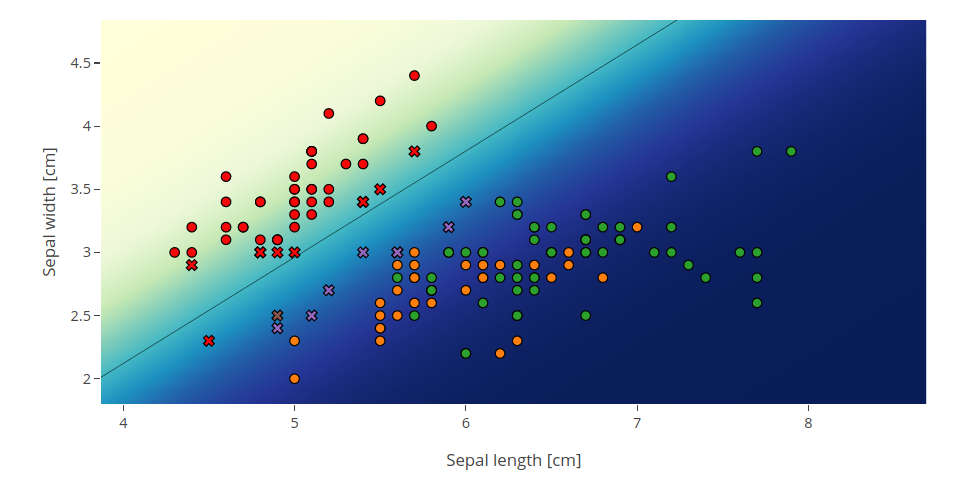
\includegraphics[height=8cm]{IrisLin001_1}
	\caption{Small Epsilon (0.001) in combination with small C shifts the decision boundary evenly between the two classes that are to be separated. The support vectors are displayed as crosses. Based on these vectors, the boundary is drawn.}
	\label{fig:smalleps}%
\end{figure}

\begin{figure}
	\centering
	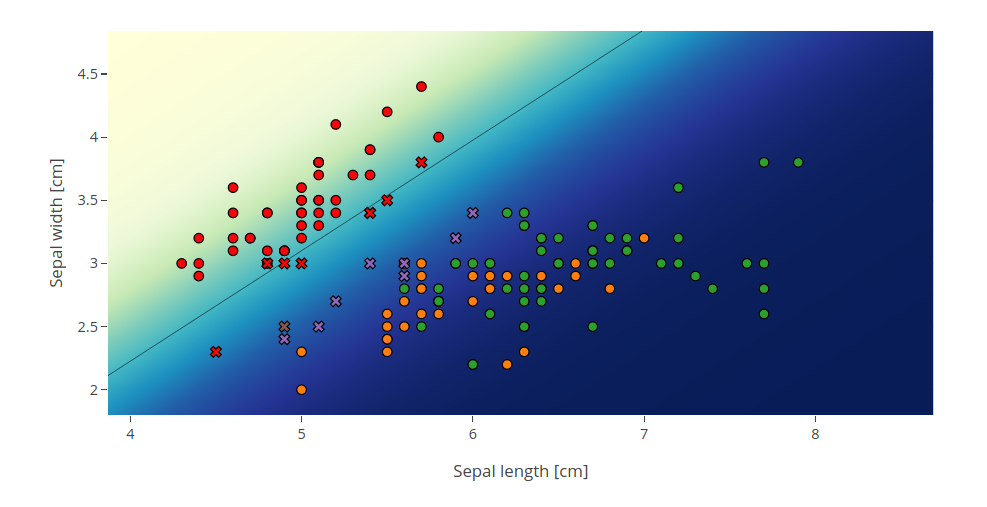
\includegraphics[height=8cm]{IrisLin51}
	\caption{Large Epsilon (0.5) shifts the decision boundary too far into the red cluster. This is due to the parameter Epsilon regulating how much influence each datapoint is assigned to, to move the decision boundary. In this case, the choice of parameters is not optimal, nevertheless most datapoints from the red cluster are classified correctly.}%
	\label{fig:largeeps}%
\end{figure}

\subsubsection*{C}
The $C$ parameter trades off correct classification of training examples against maximization of the decision function’s margin. For larger values of $C$, a smaller margin will be accepted if the decision function is better at classifying all training points correctly. A lower $C$ will encourage a larger margin, therefore a simpler decision function, at the cost of training accuracy. In other words: $C$ behaves as a regularization parameter in the SVM. 
As you can see in Figures \ref{fig:smallc} and \ref{fig:largec}
when applying larger values for $C$,
the support vectors move farther away from the decision boundary.
Support vectors are displayed as X's.

\begin{itemize}
	\item \textbf{Small $C$} makes the constraints easy to ignore which leads to a large margin
	\item \textbf{Large $C$} allows the constraints hard to be ignored which leads to a small margin
	\item For \textbf{$C = \infty$}, all the constraints are enforced.
\end{itemize}

\begin{figure}
	\centering
	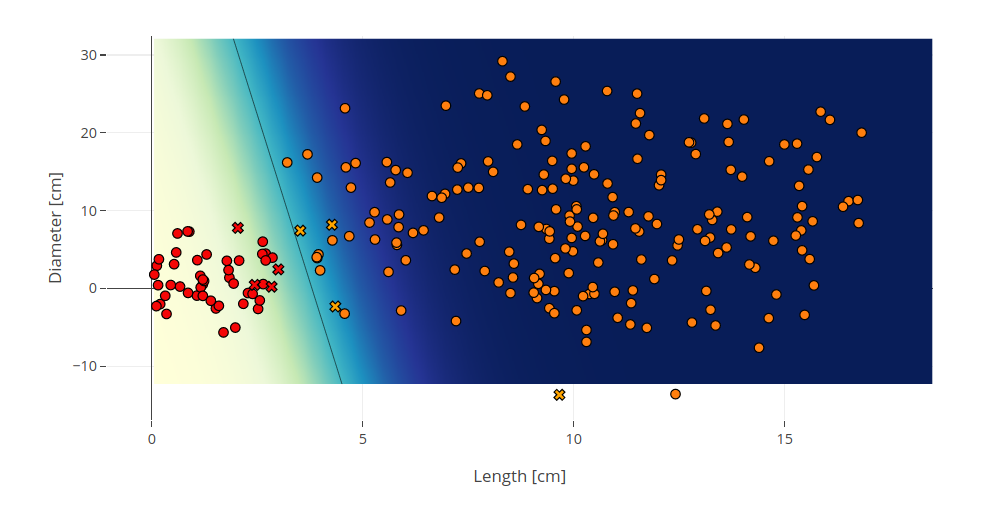
\includegraphics[height=8cm]{SalmonLin75_1}
	\caption{When picking a small value ($\approx 1$) for the C parameter in combination with a large Epsilon (0.75) the decision boundary is placed correctly balanced between the two classes.}
	\label{fig:smallc}%
\end{figure}

\begin{figure}
	\centering
	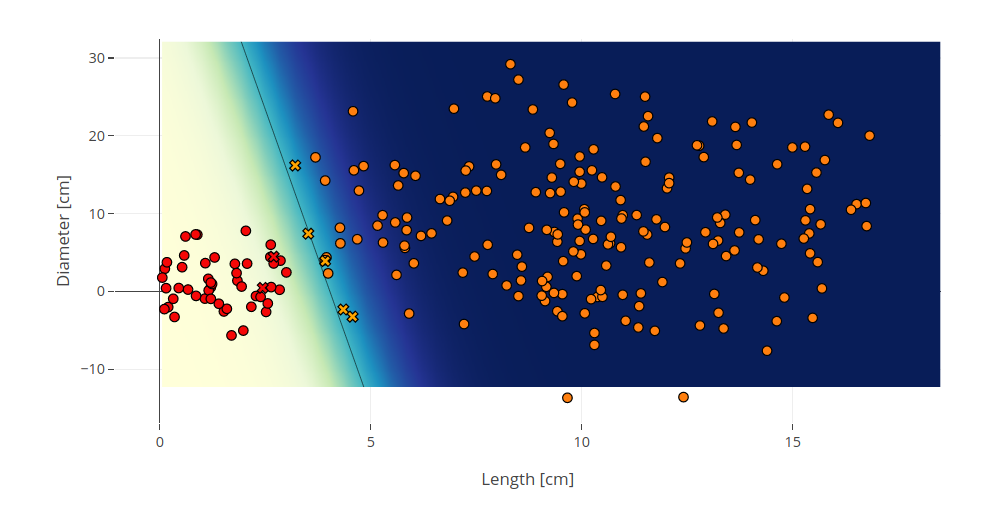
\includegraphics[height=8cm]{SalmonLin75_10k}
	\caption{With an increasingly large C parameter (C=10.000) the decision boundary may move too much towards one of the class clusters. In this example, the prediction of the orange datapoints is still correct, yet it is clearly visible that some data points are dangerously close to the decision boundary.}%
	\label{fig:largec}%
\end{figure}

\subsubsection*{Plot style}
Two different styles are available to chose from in our application: “Lines” and “Heatmap”. The \textit{Lines}-style shows the pure data in a coordinate system with plain white background. While the \textit{Heatmap}-style not only displays the data points and the separating hyperplane, but also the colored background areas.

\subsection{Explanation Tabs}

Below the SVM output, an explanation of SVMs is given.
This explanation is split across multiple tabs
that can be stepped through with the “forward” button.

\newpage
\section{Solved Challenges}

While working on this project, several challenges were overcome.

We needed to decide on which technology would be the most suitable for plotting our SVM output in the application. The two most common JavaScript frameworks for visualizing data, D3.js and Plotly.js, both seem to be similar in functionality and usability. Yet while experimenting with both frameworks, Plotly.js emerged as the more versatile and customizable software. Building upon D3.js, plotly offers a better developing experience due to its standard pipelines and configurations.

The implementation of the SVM itself turned out to be a challenge, as we created a fully functional classificator out of its mathematical description\footnote{implementation is based on \textit{Support Vector Machines Succinctly} by Alexandre Kowalczyk}. The JavaScript program can either be run, per default, without interaction with \verb|main_routine()| or show a stepwise convergence with \verb|main_routine_step()|. The Kernel functions needed to be written interchangeable and expandable. Already implemented are the \textit{linear}, \textit{polynomial} and the \textit{radial basis function} Kernels.

During our search for the optimal plot configuration, we found out that creating a contour plot brings multiple advantages over drawing a line into a scatter plot for separation, as calculating the linear equation could be hard if not impossible, if non-linear Kernels are involved. We also discovered, that smoothing the now necessary z-axis data with the $sigmoid()$ function instead of the common $sign()$ achieves way better results.

Finally, the actual data sets needed to be chosen for their representability in a tool meant for learning. This means the sets should neither have too much or too few data points, don't have too many dimensions and must be distinctly separable by the SVM. Following these constraints, we decided early on to include the well known \textit{Fischers Iris data set} into the application for its properties. Yet, after testing numerous different, publicly available, data sets, no other match was found. To offer at least one other set of data, we wrote our own data generator in python which produced the \textit{Salmon} set.

\section{Conclusion \& Future Work}

We created a fully functional SVM visualization tool
that can help build understanding of how an SVM works.
In creating these tools, we overcame or circumvented arising implementation challenges,
such as by selecting appropriate visualization frameworks.

However, the visualization software is far from complete,
and ample opportunity for future work remains
such as implementing more kernel functions or enhancing the GUI.

In particular, the current implementation runs the SVM until convergence
and then visualizes the final classification.
In the future, this could be extended
to step through the SVM one iteration at a time
in order to watch the SVM's separating boundary converge to the optimal boundary.
The SVM implementation has already been designed with the necessary hooks,
but the user interface would require additional controls for stepping.

Another possible extension involves the margins of the separating boundary.
This boundary is difficult to draw in the general case since it has no analytical form,
which is also why the user interface approximates it via a two-level contour plot.
But the boundary and with it the margins could be calculated and drawn
for the case of the linear kernel.

All in all, we have developed a well-functioning interactive tool to describe the SVM technique.
We hope that it helps people learn about SVMs,
and that it can possibly serve as the basis for future work on SVM visualization.



\end{document}
